%% LyX 2.1.3 created this file.  For more info, see http://www.lyx.org/.
%% Do not edit unless you really know what you are doing.
\documentclass{article}\usepackage[]{graphicx}\usepackage[]{color}
%% maxwidth is the original width if it is less than linewidth
%% otherwise use linewidth (to make sure the graphics do not exceed the margin)
\makeatletter
\def\maxwidth{ %
  \ifdim\Gin@nat@width>\linewidth
    \linewidth
  \else
    \Gin@nat@width
  \fi
}
\makeatother

\definecolor{fgcolor}{rgb}{0.345, 0.345, 0.345}
\newcommand{\hlnum}[1]{\textcolor[rgb]{0.686,0.059,0.569}{#1}}%
\newcommand{\hlstr}[1]{\textcolor[rgb]{0.192,0.494,0.8}{#1}}%
\newcommand{\hlcom}[1]{\textcolor[rgb]{0.678,0.584,0.686}{\textit{#1}}}%
\newcommand{\hlopt}[1]{\textcolor[rgb]{0,0,0}{#1}}%
\newcommand{\hlstd}[1]{\textcolor[rgb]{0.345,0.345,0.345}{#1}}%
\newcommand{\hlkwa}[1]{\textcolor[rgb]{0.161,0.373,0.58}{\textbf{#1}}}%
\newcommand{\hlkwb}[1]{\textcolor[rgb]{0.69,0.353,0.396}{#1}}%
\newcommand{\hlkwc}[1]{\textcolor[rgb]{0.333,0.667,0.333}{#1}}%
\newcommand{\hlkwd}[1]{\textcolor[rgb]{0.737,0.353,0.396}{\textbf{#1}}}%

\usepackage{framed}
\makeatletter
\newenvironment{kframe}{%
 \def\at@end@of@kframe{}%
 \ifinner\ifhmode%
  \def\at@end@of@kframe{\end{minipage}}%
  \begin{minipage}{\columnwidth}%
 \fi\fi%
 \def\FrameCommand##1{\hskip\@totalleftmargin \hskip-\fboxsep
 \colorbox{shadecolor}{##1}\hskip-\fboxsep
     % There is no \\@totalrightmargin, so:
     \hskip-\linewidth \hskip-\@totalleftmargin \hskip\columnwidth}%
 \MakeFramed {\advance\hsize-\width
   \@totalleftmargin\z@ \linewidth\hsize
   \@setminipage}}%
 {\par\unskip\endMakeFramed%
 \at@end@of@kframe}
\makeatother

\definecolor{shadecolor}{rgb}{.97, .97, .97}
\definecolor{messagecolor}{rgb}{0, 0, 0}
\definecolor{warningcolor}{rgb}{1, 0, 1}
\definecolor{errorcolor}{rgb}{1, 0, 0}
\newenvironment{knitrout}{}{} % an empty environment to be redefined in TeX

\usepackage{alltt} 
\usepackage{ucs}
\usepackage[utf8x]{inputenc}
\usepackage[sc]{mathpazo}
\usepackage[T1]{fontenc}
\usepackage{geometry}

\geometry{verbose,tmargin=2.5cm,bmargin=2.5cm,lmargin=2.5cm,rmargin=2.5cm}
\setcounter{secnumdepth}{2}
\setcounter{tocdepth}{2}
\usepackage{url}
\usepackage[unicode=true,pdfusetitle,
 bookmarks=true,bookmarksnumbered=true,bookmarksopen=true,bookmarksopenlevel=2,
 breaklinks=false,pdfborder={0 0 1},backref=false,colorlinks=false]
 {hyperref}
\hypersetup{
 pdfstartview={XYZ null null 1}}
\IfFileExists{upquote.sty}{\usepackage{upquote}}{}
\begin{document}



\title{42.AMO 6.\ klases rezultāti}

\author{}
\date{}

\maketitle

\section{Dalībnieku aktivitāte}

Šajā sadaļā atbildēsim uz jautājumu, kāda daļa no 6.klasei atbilstošās vecuma grupas skolēniem piedalījās 42.\ AMO. 
Dati par skolēnu skaitu pa re\v{g}ioniem, klasēm un mācību valodām ņemti no IZM publiskotās statistikas --- \url{http://izm.gov.lv/lv/publikacijas-un-statistika/statistika-par-visparejo-izglitibu/2014-2015-m-g}. Dati apkopoti par 9 lielajām pilsētām kā arī par re\v{g}ioniem, kuros nav ietvertas lielās pilsētas. Ar {\em re\v{g}ioniem} domāti NUTS3 re\v{g}ioni --- sk. \url{http://en.wikipedia.org/wiki/Statistical_regions_of_Latvia} - Kurzeme, Latgale, Pierīga Rīga, Vidzeme, Zemgale.

Olimpiādes darba valodu esam noteikuši, aplūkojot katra konkrētā darba risinājumā izmantoto valodu. (Gadījumos, kad pašu darbu neredzējām, aplūkojām skolēna re\v{g}istrācijā minēto informāciju, bet nere\v{g}istrētiem dalībniekiem --- viņu skolas/skolotāja audzēkņu pārsvarā lietoto valodu.) Skolēna dzimumu noteicām pēc viņa vai viņas vārda.  

\subsection{Dalība no 1000 skolas vecuma bērniem}



% Varbūt arī pa 6 NUTS regioniem - visi/latvieši/krievi

\begin{knitrout}
\definecolor{shadecolor}{rgb}{0.969, 0.969, 0.969}\color{fgcolor}

{\centering 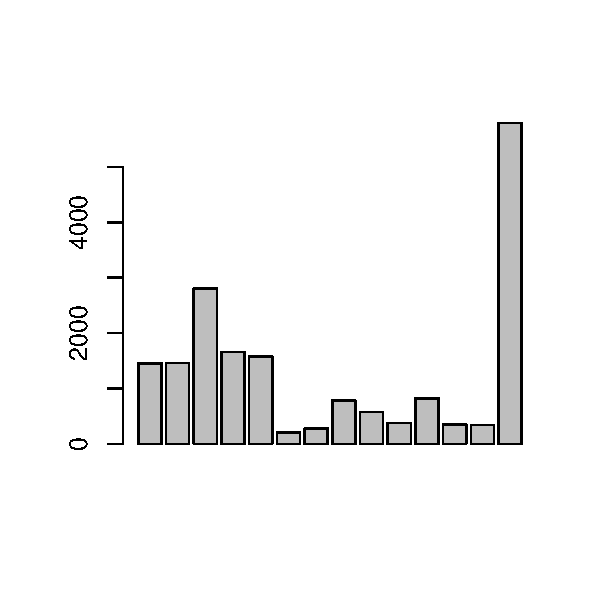
\includegraphics[width=\maxwidth]{figure/minimal-grade6-barplot-1} 

}



\end{knitrout}

% 1+9+5 aktivitāšu skaitļi pa reģioniem
% Katram no 15 reģioniem dota dzimumu proporcija
%% Stabiņi grupās pa 3 - visi/meitenes/zēni. 

% 1+9+5 aktivitāšu skaitļi pa reģioniem - darbi latviešu valodā
% Katram no 15 reģioniem dota dzimumu proporcija

% 1+9+5 aktivitāšu skaitļi pa reģioniem - darbi krievu valodā
% Katram no 15 reģioniem dota dzimumu proporcija

\subsection{Dalība un sociāli-ekonomiskie rādītāji}

% Trīs 14-bumbulīšu diagrammas
% Bezdarbs
% IIN uz 1 iedzīvotāju
% Izdevumi uz 1 skolēnu


\subsection{Dalībnieku struktūra}


%% Marimekko diagrammas - dalībnieku struktūra
% https://learnr.wordpress.com/2009/03/29/ggplot2_marimekko_mosaic_chart/

%% Segmenti -- 4 urbanizācijas tipi (LV-meitenes, LV-zēni, RU-meitenes, RU-zēni)

%% Segmenti -- 6 NUTS reģioni
% http://en.wikipedia.org/wiki/Statistical_regions_of_Latvia







\section{Dalībnieku aktivitāte novados}

Šoreiz salīdzinām ar PMLP statistiku pa novadiem. 

% Novadu aktivitāte dilstošā secībā un saraksts

% Novadu kartes...





\section{Vidējie rezultāti dalībnieku kategorijām}

Vidējais rezultāts atkarībā no dzimuma, valodas, 
urbanizācijas tipa. Katrai dalībnieku kategorijai dota
rezultātu punktu histogramma (vērtības 0--50), vidējā vērtība
$\mu$ un standartnovirze $\sigma$. 

%% Visu dalībnieku darbi, iekrāsotas godalgotās vietas 
%% Meiteņu un zēnu darbi (Meitenes zīmējam tanī pašā histogrammā)
%% Meitenes ir sazīmētas apakšā. 

%% Urbaniz. tips. Rīgas, 8 lielo pilsētu, mazpilsētu un lauku darbi

%% Latviešu un krievu valodā rakstītie darbi

%% Latviešu un krievu valodā rakstītie darbi -- tikai 9 lielajās pilsētās


\section{Skolas un skolotāji}

% Skolas pēc dalībnieku skaita

% Skolas pēc savāktajiem punktiem

%% Skolotāji pēc dalībnieku skaita

%% Skolotāji pēc savākto punktu skaita


\section{Rakstīšanas ilgums un rezultāti}

Daudzās risināšanas telpās dežuranti atzīmēja darba nodošanas laiku. Šeit vizualizējam izplatītākos darbu rakstīšanas ilgumus (nodošanas laiks mīnus 10:30) un dalībnieka rezultāta atkarību no rakstīšanas ilguma.


% Rakstīšanas ilgumu histogramma (15 min. intervāli)


% Vidējais rezultāts atkarībā no rakstīšanas ilguma


% Cik ilgi olimpiādes darbu rakstījuši bērni atkarībā no rezultāta
% 1-3 vietu ieguvēji, atzinību ieguvēji, utt. 


% Cik ilgi olimpiādes darbu rakstījuši bērni atkarībā no dzīvesvietas
% Dalām 14 kategorijās. 


\section{Dati par atsevišķajiem uzdevumiem}


% Vidējais rezultāts un vērtējumu sadalījums
%% 

% Uzdevumā saņemto punktu daļa dažādu kategoriju dalībnieku rezultātos

% Biseriālās korelācijas koeficienti



\begin{knitrout}
\definecolor{shadecolor}{rgb}{0.969, 0.969, 0.969}\color{fgcolor}\begin{kframe}
\begin{alltt}
\hlkwd{set.seed}\hlstd{(}\hlnum{1121}\hlstd{)}
\hlstd{(x}\hlkwb{=}\hlkwd{rnorm}\hlstd{(}\hlnum{20}\hlstd{))}
\end{alltt}
\begin{verbatim}
##  [1]  0.1449583  0.4383221  0.1531912  1.0849426  1.9995449 -0.8118832  0.1602680
##  [8]  0.5858923  0.3600880 -0.0253084  0.1508809  0.1100824  1.3596812 -0.3269946
## [15] -0.7163819  1.8097690  0.5084011 -0.5274603  0.1327188 -0.1559430
\end{verbatim}
\begin{alltt}
\hlkwd{mean}\hlstd{(x);}\hlkwd{var}\hlstd{(x)}
\end{alltt}
\begin{verbatim}
## [1] 0.3217385
## [1] 0.5714534
\end{verbatim}
\end{kframe}
\end{knitrout}

The first element of \texttt{x} is 0.1449583. Boring boxplots
and histograms recorded by the PDF device:

\begin{knitrout}
\definecolor{shadecolor}{rgb}{0.969, 0.969, 0.969}\color{fgcolor}\begin{kframe}
\begin{alltt}
\hlcom{## two plots side by side (option fig.show='hold')}
\hlkwd{par}\hlstd{(}\hlkwc{mar}\hlstd{=}\hlkwd{c}\hlstd{(}\hlnum{4}\hlstd{,}\hlnum{4}\hlstd{,}\hlnum{.1}\hlstd{,}\hlnum{.1}\hlstd{),}\hlkwc{cex.lab}\hlstd{=}\hlnum{.95}\hlstd{,}\hlkwc{cex.axis}\hlstd{=}\hlnum{.9}\hlstd{,}\hlkwc{mgp}\hlstd{=}\hlkwd{c}\hlstd{(}\hlnum{2}\hlstd{,}\hlnum{.7}\hlstd{,}\hlnum{0}\hlstd{),}\hlkwc{tcl}\hlstd{=}\hlopt{-}\hlnum{.3}\hlstd{,}\hlkwc{las}\hlstd{=}\hlnum{1}\hlstd{)}
\hlkwd{boxplot}\hlstd{(x)}
\hlkwd{hist}\hlstd{(x,}\hlkwc{main}\hlstd{=}\hlstr{''}\hlstd{)}
\end{alltt}
\end{kframe}

{\centering 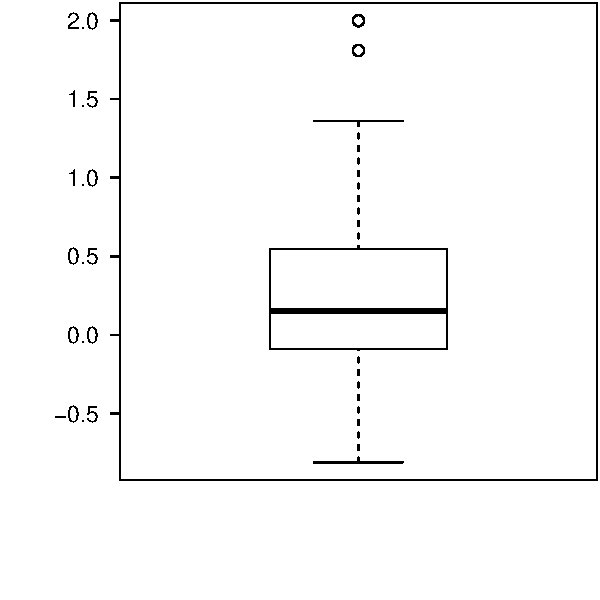
\includegraphics[width=.4\linewidth]{figure/minimal-boring-plots-1} 
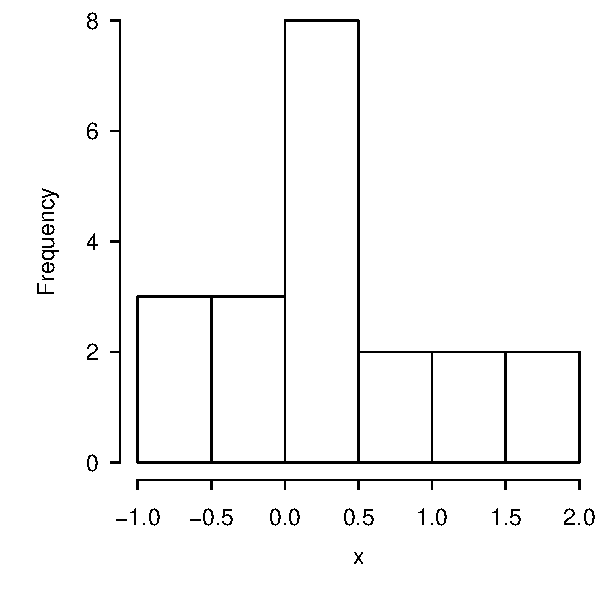
\includegraphics[width=.4\linewidth]{figure/minimal-boring-plots-2} 

}



\end{knitrout}

Do the above chunks work? You should be able to compile the \TeX{}
document and get a PDF file like this one: \url{https://github.com/yihui/knitr/releases/download/doc/knitr-minimal.pdf}.
The Rnw source of this document is at 
\end{document}
